\documentclass{beamer}
\usetheme{Madrid}
\usepackage[T1]{fontenc}
\usepackage{mathpazo}
\usepackage{graphicx}
\usepackage{booktabs}
\usepackage{tikz}
\usetikzlibrary{positioning,arrows.meta,shapes.geometric,fit,backgrounds,calc}
\definecolor{cetnavy}{RGB}{10,26,63}
\definecolor{cetlight}{RGB}{225,231,242}
\setbeamercolor{structure}{fg=cetnavy}
\setbeamercolor{frametitle}{bg=cetnavy,fg=white}
\setbeamercolor{title}{bg=cetnavy,fg=white}
\setbeamertemplate{navigation symbols}{}
% =====================================================================
%  EDIT YOUR DETAILS HERE — this ONE file feeds every abstract & deck.
%  (Change a value, recompile; all 36 documents update.)
% =====================================================================
\newcommand{\seminarName}{Aflah Muhammed P}      % <-- your full name (guessed from your email; please verify)
\newcommand{\seminarRoll}{TVE00CS000}            % <-- your university register/roll number
\newcommand{\seminarClassRoll}{00}               % <-- your class roll no (the short one)
\newcommand{\seminarGuide}{Prof.\ <Guide Name>}  % <-- your guide
\newcommand{\seminarDept}{Department of Computer Science and Engineering}
\newcommand{\seminarCollege}{College of Engineering Trivandrum}
\newcommand{\seminarShortCollege}{CET}           % shown in the slide footer, e.g. "Aflah Muhammed P (CET)"
\newcommand{\seminarShortTitle}{B.Tech Seminar}  % middle of the slide footer
\newcommand{\seminarDate}{July 31, 2026}
% ---------------------------------------------------------------------
% Optional: put a logo image named  cet_logo.png  in this folder and it
% will appear on every title slide automatically. If absent, it is skipped.
% =====================================================================

\title[\seminarShortTitle]{AgentRewardBench: Evaluating Automatic Evaluators of Web Agents}
\author[\seminarName\ (\seminarShortCollege)]{\seminarName \\ \seminarRoll \\ Roll No: \seminarClassRoll \\ Guide: \seminarGuide}
\institute[\seminarShortCollege]{\seminarDept \\ \seminarCollege}
\date{\seminarDate}
\titlegraphic{\IfFileExists{cet_logo.png}{\includegraphics[height=1.1cm]{cet_logo.png}}{}}
\begin{document}
\begin{frame}\titlepage\end{frame}
\begin{frame}{Table of Contents}\tableofcontents\end{frame}
\section{Introduction}
\begin{frame}{Introduction}
\begin{itemize}
\item Web agents automate tasks on real websites.
\item Tasks: shopping, forms, search, workflows.
\item Judging task success is surprisingly hard.
\item Rule-based checks compare final states or strings.
\item LLM judges increasingly used as scalable evaluators.
\end{itemize}
\end{frame}

\begin{frame}{The Evaluation Gap}
\textbf{\textit{Core question}}
\begin{itemize}
\item Human review is accurate but does not scale.
\item Automatic evaluators drive benchmarks and reward signals.
\item Wrong scores mislead research and training.
\item Are the evaluators themselves reliable?
\end{itemize}
\end{frame}

\section{Literature Survey}
\begin{frame}{Related Work}
\begin{itemize}
\item WebArena, VisualWebArena: realistic web benchmarks.
\item WorkArena: enterprise workflow tasks.
\item AssistantBench: open-web information tasks.
\item LLM-as-a-judge popular for open-ended outputs.
\item Prior work rarely validates the judges themselves.
\end{itemize}
\end{frame}

\section{Motivation}
\begin{frame}{Motivation}
\begin{itemize}
\item Rule-based checks are brittle and overly strict.
\item Valid alternative solutions get marked as failures.
\item LLM judges may over-credit incomplete trajectories.
\item No gold standard existed to compare evaluators.
\item Need expert labels across many settings.
\end{itemize}
\end{frame}

\section{Problem Statement}
\begin{frame}{Problem Statement}
\begin{itemize}
\item Do automatic evaluators match expert judgments?
\item Quantify agreement of rule-based and LLM judges.
\item Cover diverse benchmarks, agents, task types.
\item Measure precision and recall against expert gold.
\end{itemize}
\end{frame}

\section{Objectives}
\begin{frame}{Objectives and Contributions}
\begin{itemize}
\item Build expert-annotated trajectory benchmark (1,302 items).
\item Span 5 benchmarks and 4 agent LLMs.
\item Evaluate 12 LLM judges plus rule-based checks.
\item Expose weaknesses of current evaluation methods.
\item Guide design of more flexible evaluators.
\end{itemize}
\end{frame}

\section{Methodology Overview}
\begin{frame}{Methodology Overview}
\begin{center}
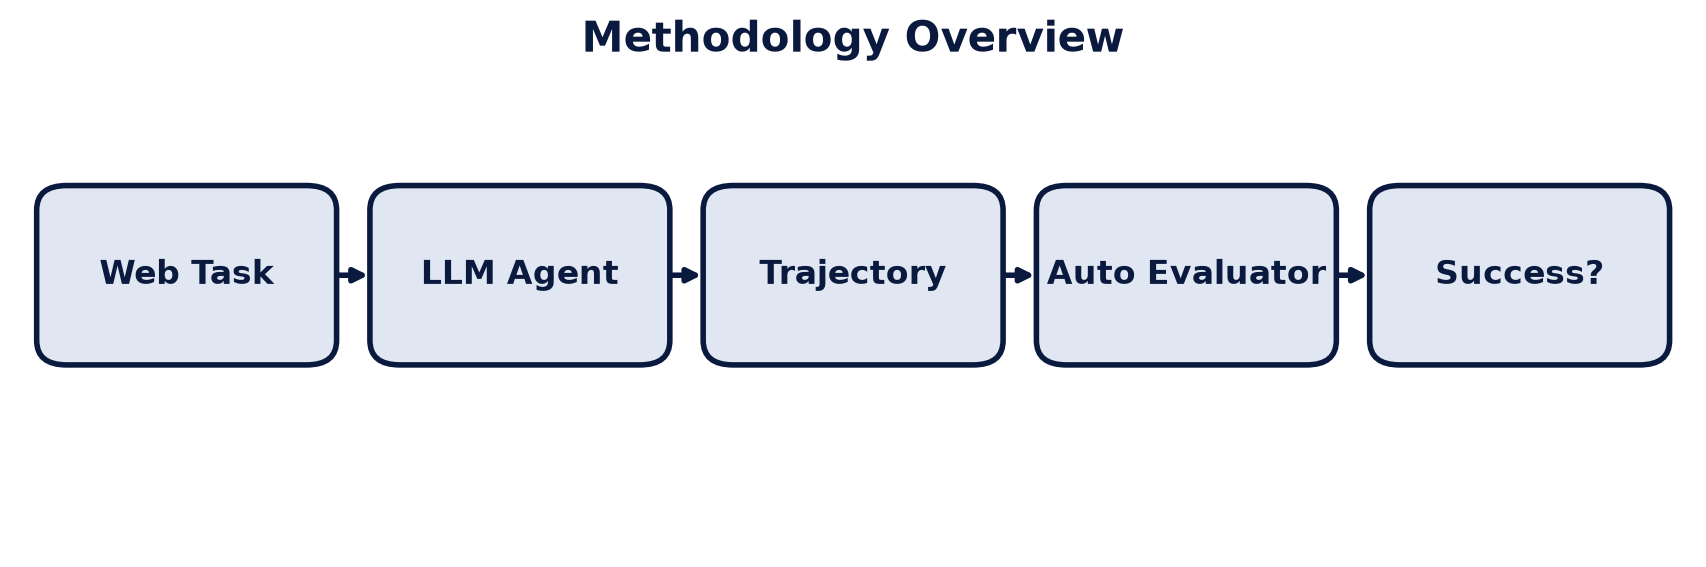
\includegraphics[width=0.9\textwidth,height=0.62\textheight,keepaspectratio]{images/agentrewardbench_1.png}
\end{center}
\end{frame}

\begin{frame}{From Trajectory to Judgment}
\begin{itemize}
\item Run agents; record screenshots and actions.
\item Experts label each trajectory as gold.
\item Apply each evaluator to same trajectory.
\item Compare evaluator output against expert label.
\end{itemize}
\end{frame}

\section{System Architecture}
\begin{frame}{System Architecture}
\begin{center}
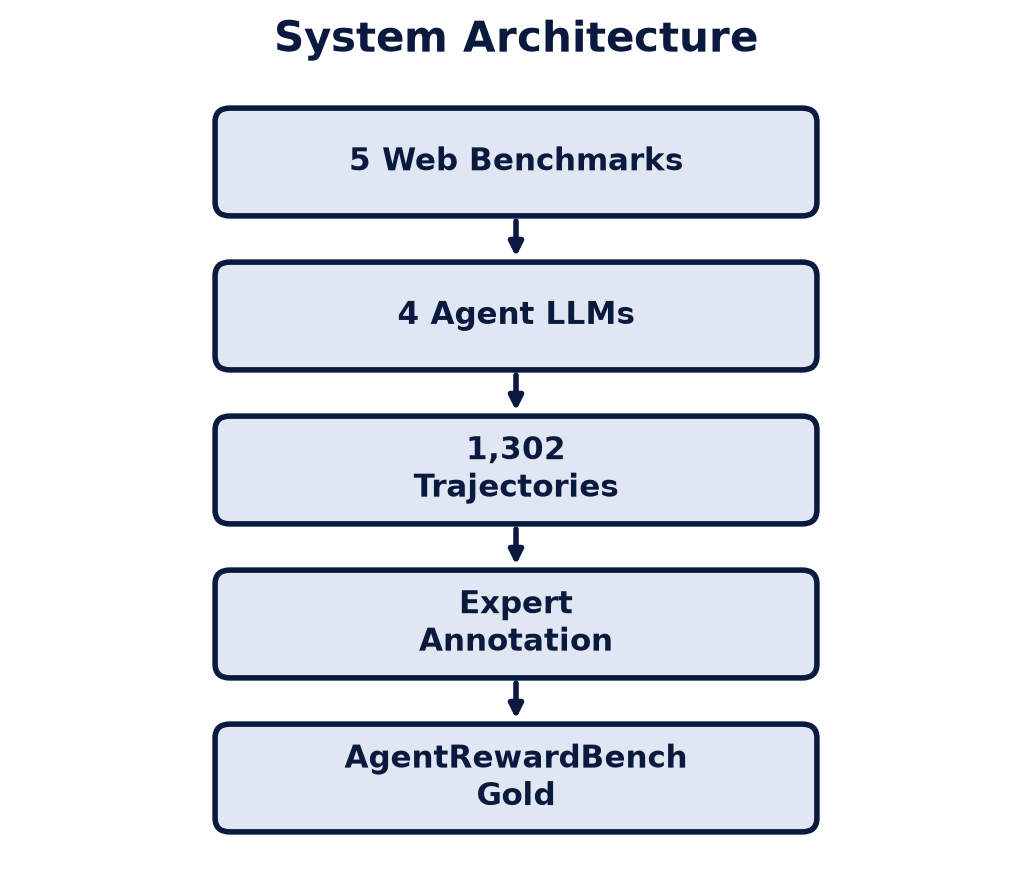
\includegraphics[width=0.9\textwidth,height=0.62\textheight,keepaspectratio]{images/agentrewardbench_2.png}
\end{center}
\end{frame}

\begin{frame}{Annotation Dimensions}
\begin{itemize}
\item Success: did the agent complete the task?
\item Side effects: unintended or harmful actions.
\item Repetition: needless repeated or looping steps.
\item Labels form the gold reference for evaluators.
\end{itemize}
\end{frame}

\section{Data Collection}
\begin{frame}{Benchmarks and Trajectories}
\begin{itemize}
\item WebArena and VisualWebArena environments.
\item WorkArena L1 and L2 workflow tasks.
\item AssistantBench open-web tasks.
\item Agents: GPT-4o, Claude 3.5 Sonnet, Llama 3.1 405B, Qwen 2.5 VL.
\item Each of 1,302 trajectories expert-reviewed.
\end{itemize}
\end{frame}

\section{Model Development}
\begin{frame}{Evaluators Under Test}
\begin{itemize}
\item Rule-based: benchmark-defined success checks.
\item LLM judges: 12 configurations prompted to score.
\item Inputs: task, actions, screenshots or accessibility tree.
\item Output: binary success prediction per trajectory.
\end{itemize}
\end{frame}

\begin{frame}{Evaluator Comparison}
\begin{center}
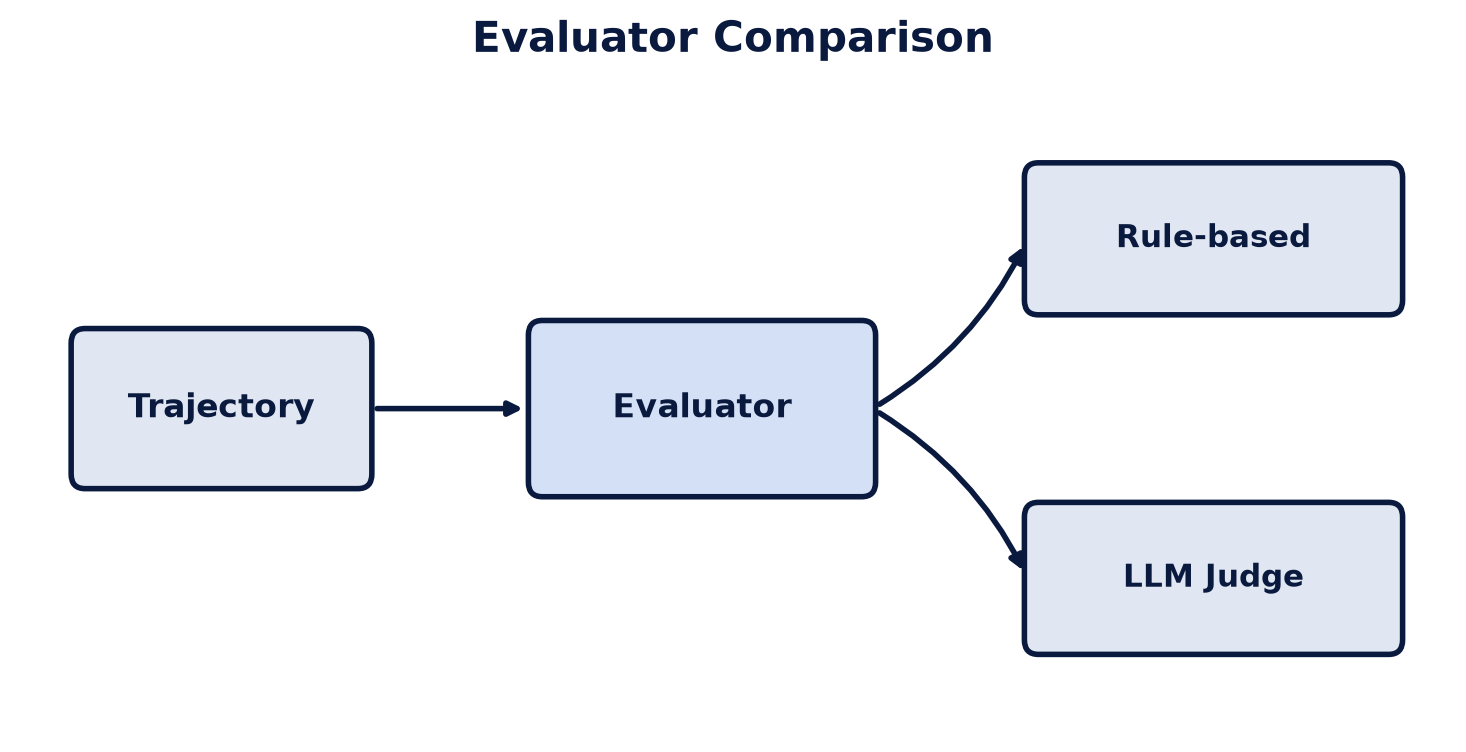
\includegraphics[width=0.9\textwidth,height=0.62\textheight,keepaspectratio]{images/agentrewardbench_3.png}
\end{center}
\end{frame}

\section{Results}
\begin{frame}{Key Results}
\begin{center}
\begin{tabular}{lcc}
\toprule
Evaluator & Precision & Recall \\
\midrule
Rule-based & High & Low \\
LLM judge (best) & High & Higher \\
o4-mini judge & Very high & Low \\
\bottomrule
\end{tabular}
\end{center}
\begin{itemize}
\item Rule-based under-reports true agent success.
\item No single LLM judge best on all benchmarks.
\end{itemize}
\end{frame}

\begin{frame}{Interpreting the Numbers}
\begin{itemize}
\item High precision, low recall means strict evaluators.
\item LLM judges recover successes rules miss.
\item Judge quality varies across benchmark and agent.
\item Evaluator choice materially changes reported success.
\end{itemize}
\end{frame}

\section{Discussions}
\begin{frame}{Discussion}
\begin{itemize}
\item Reported success rates depend on the evaluator.
\item Strict rules penalise valid alternative solutions.
\item LLM judges add flexibility but introduce bias.
\item Precision-focused judges suit reward filtering.
\item Evaluator must be reported alongside agent scores.
\end{itemize}
\end{frame}

\section{Challenges}
\begin{frame}{Challenges and Limitations}
\begin{itemize}
\item Evaluators struggle with nuanced, context-heavy tasks.
\item Limited generalisation across diverse websites.
\item LLM judges may favour certain response patterns.
\item Expert annotation is costly and hard to scale.
\end{itemize}
\end{frame}

\section{Future Work}
\begin{frame}{Future Work}
\begin{itemize}
\item Design more flexible, less brittle evaluators.
\item Combine rule-based precision with LLM recall.
\item Extend coverage to more agents and domains.
\item Use reliable judges as training reward signals.
\end{itemize}
\end{frame}

\section{Conclusion}
\begin{frame}{Conclusion}
\begin{itemize}
\item AgentRewardBench audits web-agent evaluators directly.
\item 1,302 expert-labelled trajectories, 5 benchmarks, 4 agents.
\item Rule-based checks under-report agent success.
\item No LLM judge dominates across all benchmarks.
\item Calls for more flexible automatic evaluation.
\end{itemize}
\end{frame}

\section{References}
\begin{frame}{References}
\footnotesize
\begin{itemize}
\item X. H. L\`u et al., ``AgentRewardBench: Evaluating Automatic Evaluations of Web Agent Trajectories,'' arXiv:2504.08942, 2025.
\item S. Zhou et al., ``WebArena: A Realistic Web Environment for Building Autonomous Agents,'' ICLR, 2024.
\item J. Y. Koh et al., ``VisualWebArena: Evaluating Multimodal Agents on Realistic Visual Web Tasks,'' arXiv:2401.13649, 2024.
\end{itemize}
\end{frame}
\begin{frame}\vfill\centering{\Huge Thank You}\vfill\end{frame}
\end{document}
